% #####################################################
% #####################################################
% #####################################################
\setchapterimage[3.0cm]{figures/chap3/chapter_head}

\setchapterpreamble[u]{\margintoc}
\chapter{RF Engineering Fundamentals}\label{chap:RF_fundamentals}


\epigraph{It is not knowledge, but the act of learning, not possession but the act of getting there, which grants the greatest enjoyment.}{Carl Friedrich Gauss}

This chapter is a reminder of the essential analytic elements of RF engineering used in this manuscript. Readers already aware of the transmission line and electromagnetic network theory can skip this chapter.

We will review the fundamentals of transmission line theory (Section~\ref{sec:transmission_line}), generalities about matching systems (Section~\ref{sec:matching_systems}) and scattering parameters (Section~\ref{sec:s-parameters}). Then, we will detail some particular results concerning coaxial lines (Section~\ref{sec:coaxial_lines}) and rectangular waveguides (Section~\ref{sec:rectangular_waveguide}). 

% #####################################################
% #####################################################
% #####################################################
\section[Uniform Transmission Lines]{Uniform Transmission lines Properties}\label{sec:transmission_line}
\marginnote[*-2]{Parts of this Section are taken from the documentation of the open-source Python package \href{http://scikit-rf.org/}{scikit-rf} made by the author. More about the \href{http://scikit-rf.org/}{scikit-rf} package is given in Section~\ref{sec:OSS}.}

Once RF waves have been generated, it must be transmitted to the antennas, using suitable transmission line depending on the RF frequency and power level. The main results and properties of uniform transmission lines are reviewed in this section. The results given here are well-known and can be found in numerous textbooks such as \sidecite{Harrington2001, marcuvitz1951, Thourel1988, Collin1990, gonzalez1997, pozar2012, Orfanidis, steer2019-3} to give a personal selection.

A \textit{transmission line} is specialized structure in which an RF signal can propagate. A transmission line is defined as \textit{uniform} if its dimensions and electrical properties are identical for all planes transverse to the direction of propagation. The results listed in this section are used in the following sections of this manuscript for the design and the analysis of high power RF components.

% #####################################################
\subsection{Voltage and Current}

\begin{figure}
	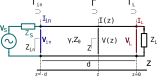
\includegraphics[width=1.0\textwidth]{figures/chap3/transmission_line_properties_vi}
	\caption{A transmission line terminated in a load impedance $Z_L$.}
	\label{fig:transmissionlinepropertiesvi}
\end{figure}

Let a lossy transmission line of propagation constant $\gamma=\alpha+j\beta$ (in [$\si{m^{-1}}$]) and characteristic impedance $Z_0$ (in [$\si{\Omega}$]), terminated by an arbitrary load $Z_L$ (in [$\si{\Omega}$]). The line length is parametrized by the distance $z$, where the source is located at distance $z=-d$ from the load (located at $z=0$) as illustrated in Figure~\ref{fig:transmissionlinepropertiesvi}. Attenuation constant $\alpha$ has the units of Nepers per meter [$\si{Np/m}$] and the phase constant $\beta$ has the units radians per meter [$\si{rad/m}$]\footnote{$1\,\si{Np/m}$ equals to $8.6859 \, \si{dB/m}$. To convert from \si{dB} to \si{Np} multiply by $0.1151$. Thus $\alpha = x \, \si{dB/m} = x \times 0.1151 \, \si{Np/m}$.}. Let $V=V(z)$ and $I=I(z)$ the total voltage and current on the line, which can be written as a sum of a forward and reflected waves:
\marginnote{$\Vfwd$ and $\Vrefl$ ($\Ifwd$ and $\Irefl$) are defined here as peak voltages (currents). For sine wave, RMS voltage is $V_{\mathrm{RMS}}=V_{\mathrm{peak}}/\sqrt{2}$.}
\begin{subequations}
\begin{align}
	V(z) = \Vfwd(z) + \Vrefl(z) =& \Vfwd e^{-\gamma z} + \Vrefl e^{+\gamma z} \\
	I(z) = \Ifwd(z) + \Irefl(z) =& \frac{\Vfwd}{Z_0} e^{-\gamma z} - \frac{\Vrefl}{Z_0} e^{+\gamma z}
\end{align}
	\label{eq:voltage_current_lossy_line}
\end{subequations}
where the $e^{-\gamma z}$ term represents wave propagation in the $+z$ direction (and $e^{+\gamma z}$ in the $-z$ direction). The terms $\Vfwd$, $\Vrefl$ ($\Ifwd$, $\Irefl$) represent the forward and reflected voltage (current) waves at $z=0$.  
The \textit{characteristic impedance} $Z_0$ associated to a uniform transmission line (or any continuous media supporting the propagation of electromagnetic waves) is defined as the ratio of the forward voltage and current when the transmission line is infinite, i.e.  $Z_0=\Vfwd/\Ifwd(=-\Vrefl/\Irefl)$. It characterizes the property of the line to oppose a change in voltage for a change of current or vice-versa. When $Z_L=Z_0$, the load is said to be \textit{matched} to the line and there is no reflected wave ($\Vrefl=0$).

\begin{marginfigure}[-2cm]
	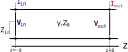
\includegraphics[width=1\linewidth]{figures/chap3/transmission_line_transfer}
	\caption{Propagation of current and voltage in a piece of uniform transmission line.}
	\label{fig:transmission_line_transfer}
\end{marginfigure}

The voltage and current at the input ($z=-d$) of a piece of uniform transmission line can be related to the voltage and current at its output (chosen at $z=0$) using the transfer matrix \sidecite{vittoria1998}:
\begin{equation}
\left( 
\begin{array}{c}
	V_{\mathrm{in}} \\
	I_{\mathrm{in}}
\end{array}
\right)
=
\left( 
\begin{array}{cc}
\cosh  \left(\gamma d\right) & Z_0 \sinh \left(\gamma d \right) \\ 
\frac{1}{Z_0}\sinh \left( \gamma d\right) & \cosh\left(\gamma d\right) 
\end{array} 
\right)
\left( 
\begin{array}{c}
	V_{\mathrm{out}} \\
	I_{\mathrm{out}}
\end{array}
\right)
	\label{eq:voltage_current_transfer_matrix}
\end{equation}




% #####################################################
\subsection{Reflection Coefficient}
The ratio of the reflected to forward voltage (or current) at a distance $z$ defines the \textit{reflection coefficient} $\Gamma$:
\marginnote{\textit{Return loss} RL is the negative of the magnitude of the reflection coefficient in \si{dB}. Since power is proportional to the square of the voltage, return loss is given by $$\mathrm{RL} = -20 \log_{10} |\Gamma|$$
The \textit{transmission coefficient} can be also defined as $$T=1+\Gamma$$
 sometime expressed as the \textit{insertion loss} IL in \si{dB}:
 $$\mathrm{IL}=-20 \log |T|$$}
\begin{equation}
\Gamma(z) = \frac{\Vrefl(z)}{\Vfwd(z)} =  \frac{\Irefl(z)}{\Ifwd(z)} = \Gamma_L e^{2\gamma z}
\label{eq:Gamma_at_z}
\end{equation}
where $\Gamma_L$ is the reflection coefficient of the load ($z=0$), given by:
\begin{equation}
	\Gamma_L = \frac{Z_L - Z_0}{Z_L + Z_0}
	\label{eq:Gamma_L}
\end{equation}
Note that the reflection coefficient at the input of the line $\Gamma_{\mathrm{in}}$ (Figure~\ref{fig:coaxial_line_fields}) is given for $z=-d$:
$$
\Gamma_{\mathrm{in}}=\Gamma(z=-d)=\Gamma_L e^{-2\gamma d}
$$

In fusion application, the load is unfortunately rarely matched to the transmission line or the source impedances, so it is convenient to re-express voltage and current equations (\ref{eq:voltage_current_lossy_line}) as a function of $\Gamma_L$ (\ref{eq:Gamma_L}) or $\Gamma(z)$ (\ref{eq:Gamma_at_z}):
\begin{subequations}
	\begin{align}
		V(z) =& \Vfwd \left( e^{-\gamma z} + \Gamma_L e^{+\gamma z} \right) 
			= \Vfwd \left[ 1 + \Gamma(z) \right]  e^{-\gamma z} \\
		I(z) =& \frac{\Vfwd}{Z_0} \left( e^{-\gamma z} - \Gamma_L e^{+\gamma z} \right)
			= \frac{\Vfwd}{Z_0} \left[ 1 - \Gamma_L(z)  \right]e^{-\gamma z}
	\end{align}
	\label{eq:voltage_current_lossy_line_gamma}
\end{subequations} 

The \textit{standing wave ratio} (SWR) is defined as:
\marginnote[*-1]{With the inverse expression
	$$ 	|\Gamma| = \frac{\SWR - 1}{\SWR + 1} $$}
\begin{equation}
	\SWR(z) = \frac{1 + |\Gamma(z)|}{1 - |\Gamma(z)|}
	\label{eq:SWR}
\end{equation}
The SWR can be equivalently defined as the ratio of maximum (forward and backward waves are in phase) to minimum (forward and reflected waves are out of phase) voltage magnitudes: 
\begin{equation}
\SWR(z) = \frac{|V_\mathrm{max}(z)|}{|V_\mathrm{min}(z)|} = \frac{|\Vfwd|e^{-\alpha z} + |\Vrefl|e^{+\alpha z}}{|\Vfwd|e^{-\alpha z} - |\Vrefl|e^{+\alpha z}}
\label{eq:SWR_max_to_min_voltages}
\end{equation}
Note that the SWR becomes constant for lossless lines. 


Finally, some special cases are recalled for convenience in the Table~\ref{tab:special_case_loaded_line}.

\begin{table}[h]
	\begin{center}
\begin{tabular}{|c|c|c|}
	\hline 
	Case & $\Gamma$ & $\SWR$ \\ 
	\hline 
	Matched: $Z_L = Z_0$ & 0 & 1 \\ 
	\hline 
	Short: $Z_L=0$ & -1 & $\infty$ \\ 
	\hline 
	Open: $Z_L = \infty$ & 1 & $\infty$ \\
	\hline
\end{tabular}
	\end{center}
\caption{Special cases of a uniform loaded transmission line.}
\label{tab:special_case_loaded_line} 
\end{table}


In the particular case of ICRH antennas, the reactance $X_s$ of the radiating elements ("straps") is generally much larger then its resistance $R_s$, i.e. $R_s \ll X_s$. Assuming a strap of impedance $Z_s=R_s+j X_s$ connected to a transmission line of real characteristic impedance $Z_0$, the SWR can approximated to:

\begin{equation}
	\SWR \approx \frac{Z_0^2 + X_s^2}{R_s Z_0}
\end{equation}



% #####################################################
\subsection{Line Impedance}
The impedance seen toward the load at a point of the line, i.e. the ratio between total voltage and current at this point, is at a distance $z=-\ell$ from the load:
\begin{subequations}
	\begin{align}
Z(z=-\ell) 
	=& Z_0 \frac{Z_L + Z_0 \tanh( \gamma \ell)}{Z_0 + Z_L \tanh(\gamma \ell)} \\
	=& Z_0 \frac{1 + \Gamma(-\ell) }{1 - \Gamma(-\ell) }
	\end{align}
\end{subequations}
As noted above with respect to Figure~\ref{fig:transmission_line_transfer}, we have in particular $Z_{\mathrm{in}}=Z(z=-d)$ and $Z(z=0)=Z_L$.

% #####################################################
\subsection{Power and losses}\label{sec:power_and_losses}
The time average power flowing along the transmission line is defined as:
\begin{equation}
P (z) = \frac{1}{2} \Re\left[V(z) I^*(z)\right] 
\label{eq:power_time_average_general}
\end{equation}

\marginnote{An example in the \href{https://scikit-rf.readthedocs.io}{scikit-rf package documentation} is dedicated to the evolution of the power, voltage, current and SWR in lossy line. See \cite[§2.7]{pozar2012}, \cite[§2.5.5]{steer2019}, \cite[§3-4c]{Rizzi1988} for discussions of power in lossy terminated line.}

For a lossy transmission line ($\alpha>0$), not all the power entering the transmission line will be delivered to the load as some power will be lost on the line due to attenuation. The time average power at any point of the transmission line (\ref{eq:power_time_average_general}) can be shown to be \sidecite[+1cm]{vernon1969, marks1992}:
\begin{subequations}
\begin{align} 
	P(z) =& P_\mathrm{f} - P_\mathrm{r} - P_\mathrm{c} \\
	P_\mathrm{f} =& \Re(Z_0) \frac{|V_\mathrm{f}|^2}{2 |Z_0|^2} e^{-2\alpha z} \\
	P_\mathrm{r} =& \Re(Z_0) \frac{|V_\mathrm{r}|^2}{2 |Z_0|^2} e^{+2\alpha z} = P_\mathrm{f} |\Gamma_L|^2 e^{+4\alpha z} \\
	P_\mathrm{c} =& \Im(Z_0) \Im\left[\frac{\Vrefl\Vfwd^*}{|Z_0|^2} e^{-2j\beta z} \right]
\end{align}
\end{subequations}
where $P_\mathrm{f}$ and $P_\mathrm{r}$ are the forward and reflected power respectively. In lossy lines, the net power flow $P(z)$ is not in general the difference of the forward and reflected power but carries an additional term $P_\mathrm{c}$. $P_\mathrm{c}$ can be either positive or negative along the line and is null for all $z$ only for a distortion-less line ($\Im(Z_0)=0$). In a word, the superposition of power does not apply in lossy uniform transmission lines (but superposition of voltages and currents does).

Keeping the notation used in Figure~\ref{fig:transmissionlinepropertiesvi} and using equations (\ref{eq:voltage_current_lossy_line_gamma}), the power delivered to the load (at position $z=0$) and at the input of the line (at position $z=-d$) are:
\begin{subequations}
	\begin{align}
		P_{\mathrm{L}} = P(z=0) =& \Re(Z_0) \frac{\left| \Vfwd \right|^2}{2 |Z_0|^2} \left(1 - |\Gamma_L|^2 \right) \\
		P_{\mathrm{in}} = P(z=-d) =& \Re(Z_0) \frac{\left| \Vfwd \right|^2}{2 |Z_0|^2} \left(1 - |\Gamma_L|^2 e^{-4\alpha d}  \right) e^{2\alpha d}
	\end{align}
\end{subequations}
hence the power lost in the line is:
\marginnote{The total loss $\mathrm{ML}$ in a line in \si{dB} can also be stated as:
$$
 \mathrm{TL}=10\log_{10} \left( \frac{A^2 - |\Gamma_L|^2}{A(1 - |\Gamma_L|^2)} \right)
$$
where $A=10^{\mathrm{ML}/10}$ and $\mathrm{ML}$ the matched line loss. The additional loss caused by the standing waves is the difference between the  $\mathrm{TL}$ and  $\mathrm{ML}$.
}
\begin{equation}
P_{\mathrm{loss}} = P_{\mathrm{in}} - P_{\mathrm{L}} 
= \Re(Z_0)  \frac{\left| \Vfwd \right|^2}{2 |Z_0|^2} 
\left[ 
\left(e^{2\alpha d} - 1\right) + |\Gamma_L|^2 \left( 1 - e^{-2\alpha d} \right)
\right]
\label{eq:power_loss_lossy_transmission_line}
\end{equation}
where the first and second terms in (\ref{eq:power_loss_lossy_transmission_line}) account for the power loss of the forward and reflected waves respectively.
	


For lossless transmission line and real characteristic impedance, the time average power flow along the transmission line is constant and (\ref{eq:power_time_average_general}) simplifies to:
\begin{equation}
P = P_\mathrm{f} - P_\mathrm{r} = P_\mathrm{f} \left(1 - |\Gamma_L|^2\right)
\label{eq:power_loss_lossless_transmission_line}
\end{equation}
This power can also be related to the maximum voltages or currents and $\SWR$ from Eq.(\ref{eq:SWR_max_to_min_voltages}):
\begin{equation}
P = P_\mathrm{f} - P_\mathrm{r} = \frac{1}{2 Z_0} \frac{	|V_{\mathrm{max}}|^2}{\SWR} = \frac{Z_0}{2} \frac{|I_{\mathrm{max}}|^2}{\SWR}
\label{eq:power_loss_lossless_transmission_line_maxvoltage_maxcurrent}
\end{equation}
where $|V_{\mathrm{max}}| = \max_z |V(z)| = |\Vfwd| + |\Vrefl|$ and similarly for $|I_\mathrm{max}|$. Combining the above two expressions leads to convenient formulas for heat flux and breakdown estimations, which relates the maximum (peak) voltage or current to the forward power $P_\mathrm{f}$ and reflection coefficient $|\Gamma_L|$:
\begin{subequations}
	\begin{align}
		|V_\mathrm{max}| =& \sqrt{2 Z_0 P_\mathrm{f} } \left(1 + |\Gamma_L| \right) \\
		|I_\mathrm{max}| =& \sqrt{\frac{2 P_\mathrm{f}}{Z_0} } \left(1 + |\Gamma_L| \right)
	\end{align}
	\label{eq:max_current_function_forward_power_gammaL}
\end{subequations}

The power lost in the transmission line is converted into heat in the metallic conductors and dielectric elements due to Ohmic and dielectric losses respectively. This heat must be evacuated to sustain CW operation. Before expressing loss formulas for the main two kinds of transmission lines used for ICRH and LHCD, we recall here for future references that the power loss in a good conductor can be calculated as:
\begin{equation}
P_\ell = \frac{R_s}{2} \int_S |J_s|^2 \diff S = \frac{R_s}{2} \int_S |H_t|^2 \diff S 
\label{eq:power_loss_conductor}
\end{equation}
where the integral is performed over the conductor surface(s), $J_s$ and $H_t$ are the surface current and the tangential magnetic field respectively\cite[§1.7]{pozar2012}. 

The \textit{skin depth} $\delta_s$ (in $[\si{m}]$) is defined as:
\begin{equation}
\delta_s 
	=
	\sqrt{\frac{2}{\omega \mu \sigma}}
	\label{eq:skin_depth}
\end{equation}
and the \textit{sheet resistance} $R_s$ (in $[\si{\Omega}]$) as:
\begin{equation}
R_s 
	= 
	\frac{1}{\delta_s \sigma}
	=
	\sqrt{\frac{\omega\mu}{2\sigma}}
	=
	\sqrt{\pi f \rho \mu }
	\label{eq:sheet_resistance}
\end{equation}
with $\sigma=1/\rho$ the metal conductivity (in $[\si{S/m}]$) and $\sigma$ the metal resistivity (in $[\si{\Omega m}]$). 

% #####################################################
% #####################################################
\section{Matching Systems}\label{sec:matching_systems}
In high power RF systems for fusion applications, the load is ultimately the plasma facing the antennas. As seen in Section~\ref{sec:icrh} and Section~\ref{sec:lhcd}, the plasma loading impedance is generally small compared to antenna and transmission line. Hence, a significant amount of RF power will be reflected toward the generators. It is essential to protect high power RF sources (tetrodes, klystrons) from reflected power (output mismatch). Reflected power perturbs the source impedance, the output amplitude and phase and creates higher dissipation losses\sidecite[-1cm]{pompon2012}. It can also lead to the failure of RF windows \sidecite[-+0.5cm]{ikeda1989} or even damage the tube itself\sidecite{gold1997,carter2005,benford2007}. 

Unfortunately, the plasma characteristics depend on the machine setup but also on its history, hence its RF load properties are relatively little known in advance. In addition, plasma intrinsic instabilities, such as Edge Localized Modes (ELMs), can also induce strong and fast load variations in front of the antenna, which may affect strongly the generator performances for the aforementioned reasons\sidecite{braun1995, beaumont1996} or generate breakdown in antennas and transmission lines due to peak voltage increases \sidecite{bobkov2003-1, goniche2012-2}. 

\begin{marginfigure}[*+5]
	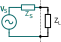
\includegraphics[width=0.8\linewidth]{figures/chap3/transmission_line_matching}
	\caption{Matching a load impedance $Z_L$ to a source having an internal impedance $Z_S$.}
	\label{fig:transmission_matching}
\end{marginfigure}

Let us consider the simplified network illustrated in Fig.\ref{fig:transmission_matching}. Classical results of RF engineering state that\cite{Rizzi1988, pozar2012}:
\begin{itemize}
	\item Conjugate Matching: maximum available power goes into the load if $Z_L=Z_S^*$
	\item Impedance Matching: minimum reflection ($\Gamma_L=0, \SWR=1$) is obtained for $Z_L=Z_S$
\end{itemize} 
As in typical plasma application the load impedance $Z_L$ is complex-valued, achieving both objectives at the same time is not possible. For this reason, a set of matching networks must be inserted between the source and the load as illustrated in Fig.~\ref{fig:transmission_matching_system}. Ideally, such a matching system should meet the following objectives (sometimes interrelated):
\begin{itemize}
	\item maximize the power transfer to the antenna 
	\item minimize the power reflected to the generator (protection and efficiency)
	\item minimize the power lost in the transmission line (net efficiency)
	\item ensure the good control of the antenna amplitude/phase
\end{itemize}

If the generator is not equipped with internal matching network, it is a good engineering practice to place a matching network as close as possible from its output. Similarly, placing a matching network as close as possible from the load reduce the standing waves and thus the peak current (dissipation problems) and the peak voltage (corona and breakdown problems) in the transmission line between the source and the load \cite[§4]{Rizzi1988}.

\begin{figure}
	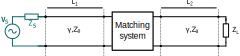
\includegraphics[width=1\linewidth]{figures/chap3/transmission_line_matching_system}
	\caption{A matching system is inserted between the source and the load impedance.}
	\label{fig:transmission_matching_system}
\end{figure}

Matching is frequency dependant since it deals with the adjustment of reactances. The perfect impedance match can occur only at one frequency but high power sources are usually very narrowband. If the source frequency can be tuned, which is the case of ICRH generators, matching networks are designed to be tunable. Such system use stub (shunt coaxial section that ends in a movable short) and line stretchers (transmission line section that can vary its electrical distance). In theory, a one-quarter-wavelength stub in conjunction with a half-wavelength stretcher can match any impedance to the generator\sidecite{england1989}. However, the actuators of these systems rely on motors (capacitors) or hydraulic systems (tuning stub, line stretchers), so their response time is of the order to 100 milliseconds or higher, which is much slower than most uncontrolled plasma variations. For this reason, fusion RF antenna are now designed to be intrinsically relatively load-tolerant, using specific feeding line or antenna design. 


% #####################################################
% #####################################################
\section{Scattering Parameters}\label{sec:s-parameters}
Voltage  $V(z)$ and current $I(z)$ as defined in Eq.(\ref{eq:voltage_current_lossy_line}) in the previous section are the "real" waves in the sense that they are linked directly to Maxwell’s equations and can be measured. For example, reflection coefficients $\Gamma(z)$ can be measured from the peaks and valleys of the electric fields of the standing wave created by the beating of forward and reflected voltages and currents in a slotted-line experiment \sidecite{marks1992, williams2013}. 

A RF \textit{network} such as the one illustrated in Fig.~\ref{fig:microwave_network}, is a system for which a closed surface separating the network from the rest of the world can be found such that it has zero current on this surface ($\hat{\mathbf{n}} \times \Ebf=0$) except over one or more input/output \textit{port} cross-section \cite[§8.3]{Harrington2001}. The electrical behaviour of linear electrical networks is often handled using impedances or admittances parameters, relating voltages to currents at each port (or reference planes). Direct measurements of these impedances or admittances of a RF network requires that the ports be terminated in either short or open circuits. However, as lead inductance and capacitance make short and open circuits difficult to obtain at RF frequencies, such terminations are often hard to realize correctly. Since power transfer is often a crucial characteristic of RF network designs, \textit{scattering parameters} (or S-parameters) are often preferred by microwave engineers since they relate the power flow of forward and reflected voltage waves at each port. Finally, scattering parameters are also well suited for describing transistors and other active devices, since short and open  terminations could result in undesired behavior, including oscillation or destruction\sidecite{steer2019-1}.

\begin{marginfigure}[*-15]
	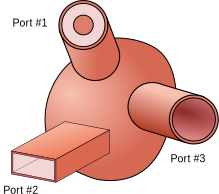
\includegraphics[width=1\linewidth]{figures/chap3/microwave_network}
	\caption{A 3 ports RF Network.}
	\label{fig:microwave_network}
\end{marginfigure}

Scattering parameters can be defined in several ways \sidecite{dobrowolski2010}, which has been discussed extensively in the literature since the 60's \sidecite{carlin1956, kurokawa1965, woods1972, marks1992, williams2013, amakawa2016}. Indeed, there is some arbitrariness to define some forward and reflected waves ($a, b$) such that ($|a|^2, |b|^2$) represent the time-averaged power carried by the forward and reflected voltage waves ($\Vfwd, \Vrefl$) (or current waves, or both). However, as seen in section \ref{sec:power_and_losses}, the power superposition principle does not hold for lossy lines and complex characteristic impedances (but superposition of voltages and currents does), so this mapping cannot be done in general. The various definitions of scattering parameters differ on how they handle complex impedances and eventually additional modes other than TEM, but all of these definitions give the same results for real-valued characteristic impedances and lossless lines\footnote{Because most of time lossless lines are assumed, this is probably the reason why most textbooks assume that the characteristic impedance is real in their presentation of scattering parameters. While complex-referenced S-parameters may be seen as a matter of purely academic concern with little practical use, it is not and it has also implications in electromagnetic simulators that are often silent on how they implement such situations.}. To deal with lossy lines and complex characteristic impedances, few methodologies exist but two are nowadays mostly adopted: \textit{power-wave} and \textit{pseudo-wave}  definitions. 

The \textit{power-waves} concept has been introduced in \sidecite{kurokawa1965}, where the forward $a$ and reflected $b$ power-waves are defined as:
\begin{subequations}
\begin{align}
	a =& \frac{V_i + Z_{R,i} I_i}{2\sqrt{|\Re(Z_{R,i})|}} \\
	b =& \frac{V_i - Z_{R,i}^* I_i}{2\sqrt{|\Re(Z_{R,i})|}}
\end{align}
\label{eq:power-waves_definition}
\end{subequations}
where $V_i$ and $I_i$ are the total voltage and current flowing into the $i$th port of the network. $Z_{i}$ is the $i$th port reference impedance. The choice of the reference impedance is free; a common practice is to set its value to the impedance of a load or a generator, enabling power waves to be used in matching problems. With power-waves, the power flowing at the port interface is:
\begin{equation}
	p_{\mathrm{pw}} = \frac{1}{2} \left( |a|^2 - |b|^2 \right)
\end{equation}

As seen in the previous section, impedance match and maximum power transfer are in general not coincident. For the latter condition, a conjugate match is required, i.e. when $Z_0 = Z_L^*$ using the notation of Fig.~\ref{fig:transmissionlinepropertiesvi}. Power-waves are defined in such a way that a conjugate match produces no reflection, and also in such a way that the incident wave carries the available power of the source and the reflected wave the total reflected power from the load\sidecite{woods1972}. Thus, the power-wave reflection coefficient is defined by:
\marginnote{To be compared with Eq.(\ref{eq:Gamma_L}).}
\begin{equation}
	\Gamma_{\mathrm{pw}} = \frac{Z_0 - Z_L^*}{Z_0 + Z_L}
\end{equation}

This definition introduces "wave" variables that can no longer be interpreted as incoming and outgoing waves from ports. However, they can be interpreted in terms of power flow at a junction, which explains its wide adoption by the RF community. Most RF circuit solvers (such as Keysight ADS, ANSYS Circuit) use the \textit{power-waves} definition. \marginnote[*-4]{Because of its wide adoption, \href{http://scikit-rf.org/}{scikit-rf} also uses the power-waves definition by default (mostly in order to replicate results from commercial solvers) but allows the use of pseudo-wave definition as well.} 

However, the power-wave definition has some caveats one must be aware of. In particular, power-waves definition may not give physical results in case of complex characteristic impedance\footnote{A simple illustration of the problem is to consider a transmission line of complex characteristic impedance $Z_0$ loaded with an impedance $Z_L=Z_0^*$. Voltage and current waves as defined at the beginning of this section will lead to a non-zero reflection coefficient $\Gamma_L$ while power-waves-based tools will give a zero reflection coefficient $\Gamma_\mathrm{pw,L}$\cite{amakawa2016}.} and are not always continuous at the interface between circuits unless reference impedance is real, so cannot be cascaded in all cases \sidecite{marks1992, williams2013}. In the real world, all transmission lines are lossy (at least to a small degree) and this contradiction has been identified shortly after \citeauthyear{kurokawa1965} seminal paper \sidecite{amakawa2016} but somewhat forgotten after. For this reason, \citeauthyear{marks1992} introduced the \textit{pseudo-waves} definition of S-parameters\footnote{where a phase factor used in \cite{marks1992} has been omitted here for simplification.}:\marginnote{Again, the pseudo-wave definition equals the travelling-wave definition when $\Zref$ is real-valued. This paragraph aims only to highlight the fact that great care should be taken when dealing with S-parameters with lossy transmission lines with electromagnetic solvers, in particular closed-source ones.}
\begin{subequations}
	\begin{align}
		a_i =& \frac{\sqrt{\Re(Z_{R,i})}}{|Z_{R,i}|} \Vfwd_i 
		= \frac{\sqrt{\Re(Z_{R,i})}}{|Z_{R,i}|} \frac{V_i + Z_{R,i} I_i}{2} \\
		b_i =& \frac{\sqrt{\Re(Z_{R,i})}}{|Z_{R,i}|} \Vrefl_i 
= \frac{\sqrt{\Re(Z_{R,i})}}{|Z_{R,i}|} \frac{V_i - Z_{R,i} I_i}{2}		
	\end{align}
\end{subequations}
where $Z_{R,i}$ is an arbitrary value which can be different from the characteristic impedance $Z_0$ of the physical transmission line at the $i$th port. $a$ and $b$ are not longer directly related to voltage and curent travelling wave and only when $Z_{R}$ equals to $Z_0$ do $a$ and $b$ correspond to actual travelling wave amplitude (normalized to unit of [$\sqrt{\si{W}}$]). The power $p$ transmitted by a pseudo-wave at the port interface is:
\begin{equation}
p = \frac{1}{2} \left(|a|^2 - |b|^2 - 2\Im(a^* b) \frac{\Im(\Zref)}{\Re(\Zref)} \right)
\end{equation}

For a N-port network, with both definitions, the forward and reflected waves are related by:
\begin{equation}
	\bbf = \Sbb \abf
\end{equation}
where the $\abf$ and $\bbf$ array are constituted of the $a_i$ and $b_i$ elements. Properties of S-matrices are discussed in \sidecite{gonzalez1997, dobrowolski2010} to name of few and are not covered here.




% #####################################################
% #####################################################
\section{Coaxial Lines}\label{sec:coaxial_lines}
% #####################################################
\subsection{Coaxial Lines Main Properties}
A coaxial line is made of two cylindrical conductors, the internal of radius $a$ and the external of radius $b$, encapsulated one inside the other as illustrated in Figure~\ref{fig:coaxial_line_geometry}. The space between both conductors is filled with a dielectric. In high power application, conductors are made of rigid metallic cylinder (aluminium or stainless steel) eventually copper or silver-coated to reduce RF losses. The dielectric is simply (dry) air, pressurized nitrogen or vacuum to reduce dielectric breakdown. 

% #####################################################
\subsection{Electric and Magnetic Fields}
The fundamental mode in a coxial line is a TEM mode as both electric and magnetic field are transverse to the propagation direction. This mode has no cut-off and therefore coaxial can be used down to DC.

\begin{marginfigure}[*-10]
	
\includegraphics[width=1\linewidth]{figures/chap3/coaxial}
	\caption{Coaxial Line Geometry}
	\label{fig:coaxial_line_geometry}
\end{marginfigure}

The electric and magnetic field inside the coaxial are illustrated in Figure~\ref{fig:coaxial_line_fields} and given by:
\begin{subequations}
	\begin{align}
		\Ebf(r) =& \frac{V}{r \ln \left(b/a \right)} \hat\ebf_r \label{eq:coaxial_electric_field}\\
		\Hbf(r) =& \frac{I}{2\pi r} \hat\ebf_\phi \label{eq:coaxial_magnetic_field}
	\end{align}
	
\end{subequations}
where $V=V_0 e^{\mp\gamma z}$ is the voltage between the conductors and $I=I_0 e^{\mp\gamma z}$ is the current in each conductor, for $a\leqslant r \leqslant b$. 

\begin{marginfigure}[*-8]
	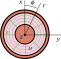
\includegraphics[width=.8\linewidth]{figures/chap3/coaxial_fields}
	\caption{TEM mode for a coaxial line}
	\label{fig:coaxial_line_fields}
\end{marginfigure}	

% #####################################################
\subsection{Characteristic Impedance}
The characteristic impedance $Z_0$ in $[\si{\Omega}]$ of a coaxial line is:
\marginnote{Or also, $Z_0\approx 138 \sqrt{\frac{\mu_r}{\varepsilon_{r}}} \log_{10}\left( \frac{b}{a} \right)$}
\begin{equation}
Z_0 = 
	\frac{1}{2\pi} \sqrt{\frac{\mu_0 \mu_r}{\varepsilon_{0} \varepsilon_{r}}} \ln\left( \frac{b}{a} \right)
	\approx
	60 \sqrt{\frac{\mu_r}{\varepsilon_{r}}} \ln\left( \frac{b}{a} \right) 
\end{equation}

with $\varepsilon_{r}$ the relative permittivity and $\mu_r$ the relative permeability of the filling dielectric. 

% #####################################################
\subsection{Power and Losses}
From Eq.(\ref{eq:coaxial_electric_field}), the maximum electric field is located on the inner conductor ($r=a$). The maximum voltage before breakdown $V_{\mathrm{max,bd}}$ is:
\begin{equation}
	V_{\mathrm{max,bd}} = a\ln\left(b/a\right) E_d
\end{equation}
where $E_d$ is the \textit{dielectric field strength} of the medium. For dry-air, this value is given as $3$~\si{MV/m} \cite[b§3.11]{pozar2012}\marginnote{The field strength in vacuum is in theory much higher. However, as detailed in Chapter~\ref{chap:Multipactor}, electrical breakdown in vacuum can occur because of other mechanisms.}. In a lossless coaxial line, the associated maximum power before breakdown $P_\mathrm{max,bd}$ is from Eq.(\ref{eq:power_loss_lossless_transmission_line}):
\begin{equation}
	P_\mathrm{max,bd} =  \frac{V^2_{\mathrm{max,bd}} }{2 Z_0 \SWR}= \sqrt{\frac{\varepsilon_{r}}{\mu_r}} \frac{a^2 E_d^2}{120\,\SWR} \ln (b/a)
\end{equation}
This expression shows that the power capability can be increased by using a larger coaxial line for the same characteristic impedance or by increasing the $b/a$ ratio (higher characteristic impedance) and by reducing the $\SWR$.

The Ohmic heat flux $\Psi$ (in [$\si{W/m^2}$]) due to the flow of RF current on a conductor of diameter $\phi$ is given by:
\begin{equation}
\Psi(\phi,z) 
=
\frac{R_s}{2}
\frac{|I(z)|^2}{(\pi \phi)^2}
\label{eq:ohmic_heat_flux_coaxial}
\end{equation}
where $R_s$ is the sheet resistance given by Eq.(\ref{eq:sheet_resistance}).

The previous expression can be used to calculate thermal behaviour of high power coaxial components (Fig.~\ref{fig:coaxial_losses}). The Ohmic power loss per unit length $P_\ell$ (in \si{W/m}) dissipated in a coaxial line is the sum of the inner and the outer conductors losses:
\begin{equation}
P_\ell (z)
=
\frac{1}{4 \pi}
\left(
\frac{R_{s,a}}{a} + \frac{R_{s,b}}{b}
\right)
|I(z)|^2
\end{equation}


\begin{figure*}
	\centering
	\includegraphics[width=0.8\linewidth]{figures/chap3/coaxial_losses}
	\caption{Coaxial losses in a 2~meter 30~\si{\Omega} 9" coaxial line with $P_\mathrm{i}=500~\si{kW}$ and  $P_\mathrm{r}=300~\si{kW}$ at 100~\si{MHz}. Inner conductor is in copper while the outer conductor is in aluminium. Heat flux from Eq.(\ref{eq:ohmic_heat_flux_coaxial}) is benchmarked against full-wave ANSYS HFSS.}
	\label{fig:coaxial_losses}
\end{figure*}

%Finally, the attenuation $\alpha=P_\ell(z=0)/(2P_0)$ in $[\si{Neper/m}]$ of a coaxial line is\cite[Ex.2.7]{pozar2012}:
%\begin{equation}
%\alpha 
%	=
%	\frac{1}{4\pi Z_0}
%	\left(
%		\frac{R_{s,a}}{a} + \frac{R_{s,b}}{b}
%	\right)
%	+
%	\frac{1}{2}\omega \varepsilon'' \eta
%\end{equation}
%where $R_{s,a}$ and $R_{s,b}$ are the sheet resistances given by eq.\ref{eq:sheet_resistance} for inner and outer conductors respectively and $\eta=\sqrt{\mu/\varepsilon'}$ is the intrinsic impedance of the dielectric material filling the coaxial line. 

% #####################################################
% #####################################################
\section{Rectangular Waveguides}\label{sec:rectangular_waveguide}
\subsection{Rectangular Waveguides Main Properties}
Electromagnetic wave can also propagate in hollow metallic structures filled with dielectric. The structure dimensions must be designed for the wavelength to transport. 

\begin{marginfigure}[0cm]
	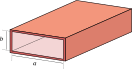
\includegraphics[width=1\linewidth]{figures/chap3/rectangular_waveguide}
	\caption{Rectangular Waveguide Geometry}
	\label{fig:rectangular_waveguide_geometry}
\end{marginfigure}

A hollow rectangular waveguide of width $a$ and height $b$ is illustrated in Figure \ref{fig:rectangular_waveguide_geometry}. Solving Maxwell’s equations for this geometry leads to multiple possible solutions, or \emph{modes}. In a rectangular waveguide, modes can be expressed as \emph{Transverse Electric} (TE) or \emph{Transverse Magnetic} (TM), depending of their respective polarization. Since the walls of a rectangular waveguide constrain the electromagnetic field boundary conditions along two dimensions, two integer indices $m$ and $n$ are used to describe a mode from another. Thus, modes in a rectangular waveguides can be $\TE_{mn}$ or $\TM_{mn}$\sidenote{With $m$ and $n$ integers greater or equal to 0 for $\TE$ modes and greater or equal to 1 for $\TM$ modes.}. These modes are eigenfunctions of the equation system and each mode is characterized by a wavenumber $\beta_{mn}$:
\begin{equation}
	\beta_{mn} = \sqrt{k^2_0 - k_{c,mn}^2 }
	\label{eq:rectwg_wavenumber}
\end{equation}
with $k_0=\omega\sqrt{\mu\varepsilon}=\sqrt{\mu_r \varepsilon_{r}}\omega/c$, where $k_{c,mn}$ is the \textit{cut-off wavenumber}:
\marginnote{We recall here for convenience that the medium wavelength $\lambda$ is:
	$$
	\lambda = \frac{\lambda_0}{n} = \frac{v_\phi}{f}
	$$
	where $\lambda_0$ is the wavelength in vacuum, $v_\phi$ is the phase velocity, $n=c/v_\phi=\sqrt{\mu_r \varepsilon_{r}}$ is the refractive index and $c=1/\sqrt{\mu_0 \varepsilon_{0}}$ the speed of light. We also define 
	$$
	\xi_0=\sqrt{\frac{\mu_0}{\varepsilon_{0}}}=120\pi=377\,\si{\Omega}
	$$ 
	as the vacuum characteristic impedance.
}
\begin{equation}
	k_{c,mn}
	=
	\sqrt{\left(\frac{m\pi}{a}\right)^{2}+\left(\frac{n\pi}{b}\right)^{2}}
	\label{eq:rectwg_cutoff_wavenumber}
\end{equation}

Each mode has an associated \textit{cut-off frequency} $f_{c,mn}$, below which a mode cannot propagate in the guide:
\begin{equation}
	f_{c,mn} = \frac{k_{c,mn}}{2\pi\sqrt{\mu \varepsilon}}
	\label{eq:rectwg_cutoff-frequency}
\end{equation}
The mode $mn$ can propagate in a rectangular waveguide only if the operating frequency is higher than the cut-off frequency of the mode, i.e. $f>f_{c,mn}$. The mode with the lowest cut-off frequency is called the \textit{fundamental} or \textit{dominant} mode. Because we have assumed that $a>b$, the lowest cut-off frequency occurs for the $\TE_{10}$ ($m=1,n=0$) mode\sidenote{There are no $\TE_{00}$ mode.}. 

For practical applications, the dimensions of the waveguides are generally chosen in order to have one and only one mode allowed propagating for a specified frequency band. Other modes can eventually be excited by waveguides discontinuities, but can’t propagate since they are evanescent ($k^2_0 < k_{c,mn}^2$ in Eq.(\ref{eq:rectwg_wavenumber})). Such modes are referred to \textit{high order modes}. For high power applications, a great care is given to waveguide inner walls, bends and connections, since reflected power and breakdowns may occur due to discontinuities in the conducting walls, such as the ones caused by flange misalignments \sidecite{harvey1955,brady1965,kerr2010}, bumps, holes, etc.

% #####################################################
\subsection{Electric and Magnetic Fields}
At a given frequency in a homogeneous-filled metallic hollow waveguide, the set of all possible TE and TM modes forms an orthogonal basis and a complete system\cite[§1.2]{marcuvitz1951},\cite[§5.2]{Collin1990},\cite[§8.2]{Harrington2001}. In practice, this sum is over all propagating modes and truncated to few evanescent modes only if needed, which is the case for antenna-plasma coupling calculations (Cf. Section~\ref{sec:lhcd}). In order to match the geometry usually used for plasma-wave coupling theory, we assume here that the large side of the waveguide is aligned in the direction $y$ and the short side in the direction of $z$. The waveguide cross-section is supposed homogenous in the $x$ direction. The geometry of a rectangular waveguide is illustrated in Fig.\ref{fig:rectangular_waveguide_geometry_fields}. The transverse electromagnetic fields can be expressed the summation of these modes:

\begin{marginfigure}[0cm]
	\includegraphics[width=1\linewidth]{figures/chap3/rectangular_waveguide_fields}
	\caption{Rectangular Waveguide Geometry and $\TE_{10}$ mode pattern derived from Eq.(\ref{eq:rectwg_EHfields_TE10})}
	\label{fig:rectangular_waveguide_geometry_fields}
\end{marginfigure}

\begin{subequations}
	\begin{align}
\mathbf{E}_{t}(\mathbf{r}) = & \sum_{p,m,n} V_{pmn}(x)\mathbf{e}_{pmn} (y,z)
\label{eq:E_guides_somme_modes}\\
\mathbf{H}_{t}(\mathbf{r}) = & \sum_{p,m,n} I_{pmn}(x)\mathbf{h}_{pmn} (y,z)
\label{eq:H_guides_somme_modes}
	\end{align}
\label{eq:rectwg_transverse_fields_sum_modes}
\end{subequations}
with $V_{pmn}$ and $I_{pmn}$ the eigenvalues of a mode $p=\{\TE,\TM\}$ of indexes $(m,n)$ and $\gamma_{pmn}=j\beta_{pmn}$ its associated wavenumber. 

\begin{subequations}
	\begin{align}
V_{pmn}(x) = & A_{pmn}e^{-\gamma_{pmn}x} + B_{pmn}e^{+\gamma_{pmn}x}
\label{eq:valeur_propre_V}\\
I_{pmn}(x) = & \frac{1}{Z_{pmn}}\left(A_{pmn}e^{-\gamma_{pmn}x} - B_{pmn}e^{+\gamma_{pmn}x}\right)
\label{eq:valeur_propre_I}
	\end{align}
	 \label{eq:rectwg_modes_eigenvalues}
\end{subequations}
with $Z_{pmn}$ the mode characteristic impedance:
\begin{equation}
Z_{pmn} = 
\begin{cases}
\frac{j\omega\mu}{\gamma_{mn}} = \frac{j k_0 \xi_0}{\gamma_{mn}} & \mathrm{\, for\, \TE\, modes}\\
\frac{\gamma_{mn}}{j\omega\varepsilon}=\frac{\gamma_{mn} \xi_0}{j k_0} & \mathrm{\, for\,\TM\, modes}
\end{cases}
\end{equation}

The modal eingenfunctions for rectangular waveguides are\cite[§2.2]{marcuvitz1951},\cite[§8.1,§8.2]{Harrington2001},\cite[§5.4]{Collin1990},\cite[§3.3]{pozar2012},\cite[Appendix A]{Bers1981} for TE modes:
\begin{eqnarray}
\mathbf{e}_{mn}^{\TE}(y,z) & = & -\ebf_x \times \mathbf{h}_{mn}^{\TE} = \ebf_x \times \nabla_{t} \psi_{mn}\\
\mathbf{h}_{mn}^{\TE}(y,z) & = &  \ebf_x \times \mathbf{e}_{mn}^{\TE} = -\nabla_{t} \psi_{mn}
\label{eq:TEmodes_eingenfunctions}
\end{eqnarray}
and for mode TM modes:
\begin{eqnarray}
\mathbf{e}_{mn}^{\TM}(y,z) & = & -\nabla_{t}\phi_{mn}\\
\mathbf{h}_{mn}^{\TM}(y,z) & = & \ebf_x \times\mathbf{e}_{mn}^{\TM}= -\ebf_x \times\nabla_{t}\phi_{mn}
\label{eq:TMmodes_eingenfunctions}
\end{eqnarray}
The longitudinal components are given by:
\begin{eqnarray}
E_{x}^{TM} & = & \sum_{m,n}\frac{k_{c,mn}^{2}}{j k_{0}}\xi_0 I_{m,n}(x)\phi_{mn}(y,z)\\
H_{x}^{TE} & = & \sum_{m,n}\frac{k_{c,mn}^{2}}{j k_{0}}\xi_0^{-1} V_{m,n}(x)\psi_{mn}(y,z)
\label{eq:TETM_longitudinal_components}
\end{eqnarray}
$\psi$ and $\phi$ are the generator functions (\emph{transverses field pattern mode functions}). For a rectangular waveguide\cite[Table 8.1]{Harrington2001}\cite[§1.2 (6.c),§2.2]{marcuvitz1951}\cite[Appendix A, A13-14]{Bers1981}:
\begin{eqnarray}
\psi_{mn} & = & \frac{1}{\pi}\sqrt{\frac{\epsilon_{m}\epsilon_{n}}{m^{2}\frac{b}{a}+n^{2}\frac{a}{b}}}\cos\left(\frac{m\pi}{a}y\right)\cos\left(\frac{n\pi}{b}z\right)\label{eq:fonction_generatrice_TE}\\
\phi_{mn} & = & \frac{2}{\pi}\sqrt{\frac{1}{m^{2}\frac{b}{a}+n^{2}\frac{a}{b}}}\sin\left(\frac{m\pi}{a}y\right)\sin\left(\frac{n\pi}{b}z\right)\label{eq:fonction_generatrice_TM}
\end{eqnarray}
where $\epsilon_{k}=1$ if $k=0$ or $\epsilon_{k}=2$ otherwise.

Since these solutions form a orthogonal basis, the following integral over the waveguide cross-section $S$ gets\cite{marcuvitz1951,Collin1990}:

\begin{equation}
\left\langle \mathbf{f},\mathbf{g}\right\rangle 
=
\iint_{S}\mathbf{f}(y,z)\mathbf{\cdot g}(y,z)\, \diff y\, \diff z
\label{eq:rectwg_scalar_product}
\end{equation}
in particular:
\begin{subequations}\label{eq:relations_orthogonalite}
	\begin{eqnarray}
	\left\langle \mathbf{e}_{mn}^{\TE},\mathbf{e}_{m'n'}^{\TE}\right\rangle  & = & \delta_{m=m',n=n'}\\
	\left\langle \mathbf{e}_{mn}^{\TE},\mathbf{h}_{m'n'}^{\TE}\right\rangle  & = & \delta_{m=m',n=n'}\\
	\left\langle \mathbf{e}_{mn}^{\TE},\mathbf{e}_{m'n'}^{\TM}\right\rangle  & = & 0\\
	\left\langle \mathbf{e}_{mn}^{\TE},\mathbf{h}_{m'n'}^{\TM}\right\rangle  & = & 0
	\end{eqnarray}
\end{subequations}
where $\delta_{m=m',n=n'}=1$ if $m=m'$ and $n=n'$, $0$ otherwise.

For the fundamental mode $\TE_{10}$ (with $a>b$), one has in particular:
\begin{subequations}
	\begin{align}
\psi_{10}(y) &= 
	\frac{1}{\pi} \sqrt{\frac{2a}{b}} \cos\left(\frac{\pi}{a} y\right) 
	\\
\Ebf_t(x,y) =& 
	-  \sqrt{\frac{2}{ab}} \sin\left(\frac{\pi}{a} y\right)V_{10}(x) \hat\ebf_z 
	\\
\Hbf_t(x,y) =& 
	   \sqrt{\frac{2}{ab}} \sin\left(\frac{\pi}{a} y\right)I_{10}(x)\hat\ebf_y 
	\\
H_x(x,y) =& 
	\frac{k_{c,10}^2}{j \omega\mu} \frac{1}{\pi} \sqrt{\frac{2a}{b}} \cos\left(\frac{\pi}{a} y\right) V_{10}(x)
	\end{align}
	\label{eq:rectwg_EHfields_TE10}
\end{subequations}
\marginnote[-3cm]{We we have used $\omega\mu=k_0\xi_0=\beta_{mn}Z_{mn}$.}

% #####################################################
\subsection{Power and Losses}
The previous choice of normalization factors leads to simple time-average power flow along a rectangular waveguide:
\begin{equation}
P=\iint\frac{1}{2}\Re\left[\mathbf{E}_{t}\times\mathbf{H}_{t}^{*}\right]\cdot \hat \ebf_x \diff S
=
\sum_{l}\frac{1}{2Z_{l}}\left(\left|A_{l}\right|^{2}-\left|B_{l}\right|^{2}\right)
\label{eq:poynting}
\end{equation}
where the sum is over the propagating modes only. 

Since the $\TE_{10}$ mode is the fundamental mode and the most used to transfer the RF power, we will specify some quantities for $m=1,n=0$. Using Eqs.(\ref{eq:rectwg_EHfields_TE10}), the power flow down the guide for the $\TE_{10}$ is:
\begin{equation}
	P_{10} = \frac{1}{2} \Re \iint_S  \left(\Ebf \times \Hbf^* \right)\cdot \hat\ebf_x \diff y \diff z
	= \frac{1}{2} \Re\left[V_{10}(x) I^*_{10}(x) \right]
	\label{eq:rectwg_poynting_TE10_V10_I10}
\end{equation}
which reads from Eqs.(\ref{eq:rectwg_modes_eigenvalues}):
\begin{equation}
	P_{10} = \frac{1}{2Z_{10}}\left(\left|A_{10}\right|^{2}-\left|B_{10}\right|^{2}\right)
	\label{eq:rectwg_poynting_TE10_A10_B10} = P_\mathrm{i} -  P_\mathrm{r}
\end{equation}
where $P_\mathrm{i}$ (in [\si{W}]) is the forward power and $P_\mathrm{r}$ the reflected power. Coefficients $|A_{10}|$ and $|B_{10}|$ can then be related conveniently to the forward and reflected power:
\begin{subequations}
	\begin{align}
	|A_{10}| =& \sqrt{2Z_{10} P_\mathrm{i}} \\
	|B_{10}| =& \sqrt{2Z_{10} P_\mathrm{r}} =  |\Gamma| |A_{10}|
	\end{align}	
\end{subequations}	
where we have used the "voltage" reflection coefficient $|\Gamma|$ defined by $\Gamma=B_{10}/A_{10}$ for a mono-mode transmission line. In practice however, the usual figure of merit is the "power" reflection coefficient given by $|\Gamma|^2 = P_\mathrm{r}/P_\mathrm{i}$. Using all the previous definitions, the electromagnetic field in Eqs.(\ref{eq:rectwg_EHfields_TE10}) can be directly related to forward and reflected powers, giving peak values comparable to full-wave calculations and for breakdown analysis. A simple benchmark of these relations is given on Fig.\ref{fig:rectwg_benchmark_fields}.

The electric field for the $\TE_{10}$ mode is maximum at $y=a/2$ (in the middle of the waveguide). This peak electric field value for this mode is:
\begin{equation}
	\left| E_{y,\mathrm{max}} \right|
	=
	2 \sqrt{\frac{Z_{10} P_\mathrm{i}}{a b }} 
		\left( 
			1 + |\Gamma|
		\right)
\end{equation}

The maximum incident power before breakdown for a given reflection coefficient in a dielectric-filled rectangular waveguide is thus:
\begin{equation}
	P_{\mathrm{max,bd}}
	= 
	\frac{a b}{4 Z_{10}} \frac{E_d^2}{\left(1 + |\Gamma|\right)^2}
\end{equation}
with $E_d$ the electric strength of the medium. The previous expression shows that the maximum power is again obtained for a minimum reflection coefficient and increase with the waveguide dimensions. 

The Ohmic loss is not homogeneous in a rectangular waveguide. The Ohmic power loss density (in [$\si{W/m^2}$]) is, for the large ($\Psi_a$) and the small ($\Psi_b$) sides of the waveguide respectively:
\begin{subequations}
	\begin{align}
		\Psi_a(x,y)
		=& \frac{R_s}{2} \left(\left| H_x(x,y) \right|^2 + \left| H_y(x,y) \right|^2 \right)
\\
		\Psi_b(x)
		=& \frac{R_s}{2} \left| H_x(x,0) \right|^2 
	\end{align}
\end{subequations}

From symmetry, the currents on the top and bottom walls are identical, as are the currents on the small walls. So, the Ohmic power loss per unit length $P_\ell$ (in \si{W/m}) for a waveguide is then: 
\begin{equation}
P_\ell (z)
= 
2\int_0^a  \Psi_a(y,z) \diff y 
+ 
2\int_0^b  \Psi_b(z) \diff z 
\end{equation}
which reads:
\begin{equation}
P_\ell (z)
= 
R_s \left[
	\frac{1}{b} \left| I_{10} \right|^2 
	+ 
	\left(
		2a + \frac{a^2}{b}
	\right)
	\frac{k_{c,10}^2}{(\omega\mu\pi)^2} 
	\left| V_{10} \right|^2 
\right]
\label{eq:rectwg_power_loss_per_unit_length}
\end{equation}

\begin{figure*}
	\centering
	\includegraphics[width=0.8\linewidth]{figures/chap3/rectangular_waveguide_fields_losses}
	\caption{$E$ and $H$ fields and RF losses in a 400~\si{mm} WR284 waveguide ($72.13 \times 34.04$~\si{mm}) with $P_\mathrm{i}=500~\si{kW}$ and  $P_\mathrm{r}=100~\si{kW}$ at 3.7~\si{GHz}. Conductor are in copper. Results are  benchmarked against full-wave ANSYS HFSS.}
	\label{fig:rectwg_benchmark_fields}
\end{figure*}


